\documentclass{article}

\usepackage[utf8]{inputenc}
\usepackage[T1]{fontenc}
\usepackage{amsmath,amssymb}
\usepackage{textcomp}
\usepackage{float}
\usepackage{listings}
\usepackage{hyperref}
\usepackage{graphicx}
\usepackage[table]{xcolor}
\usepackage{todonotes}
\usepackage{tikz}
\usepackage{pgf-umlcd}
\usetikzlibrary{positioning, fit, calc, shapes, arrows, er}

\definecolor{codegreen}{rgb}{0,0.6,0}
\definecolor{codepurple}{rgb}{0.58,0,0.82}
\definecolor{codegray}{rgb}{0.5,0.5,0.5}

\lstdefinelanguage{math}{
  keywords={var, let, in, end},
  sensitive=false,
  comment=[l]{//},
  morecomment=[s]{/*}{*/},
  morestring=[b]',
  morestring=[b]",
}

\lstdefinelanguage{xtend}{
  keywords={override, void, if, return, public, static, new, val, def, retrun, int, switch, throw},
  sensitive=false,
  comment=[l]{//},
  morecomment=[s]{/*}{*/},
  morestring=[b]',
  morestring=[b]",
}

\lstdefinestyle{wstyle}{
    keywordstyle=\color{codepurple},
    stringstyle=\color{codegreen},
    commentstyle=\color{codegray},
}

\lstset{style=wstyle}

\begin{document}

\title{Assingment 2 - External DSL Interpreter}
\author{Marc Bertelsen\\
\textbf{berte20@student.sdu.dk}}

\maketitle

\pagebreak

\section{Summary}

\begin{itemize}
    \item XText grammer - done
    \item XTend generator - done
    \item XTend validator - done
    \item XTend scoping - todo
    \item Tests \begin{itemize}
        \item MathExampleTest - all pass
        \item MathParsingTest - all pass
        \item MathScopeTest - error
        \item MathValidatorTest - all pas
    \end{itemize}
\end{itemize}

\section{Desing}

Important for the design of the metamodel and syntax, is the enforcement of mathematical operation exetuction. This has to implementated with the already given syntax from the test cases.

\subsection{Metamodel}

Fig.~\ref{fig:metamoel}, show a simple metamodel for the design of a math interpreter. By structuing the model such that the different expression sub-types share a common base class, it enables the usage of a single function for the expression computations. Additionally, the structure on the metamodel enforces the corret order of mathematical operations, by the way the expression tree is composed. Addition and subtration at the top, this will happen last in the order of operation. Multiplication and division is below, witch means they will exetuce one step before. All the Primary sub-types require even earlier computation, so they are placed deeper in the tree.

\begin{figure}[H]
    \centering
    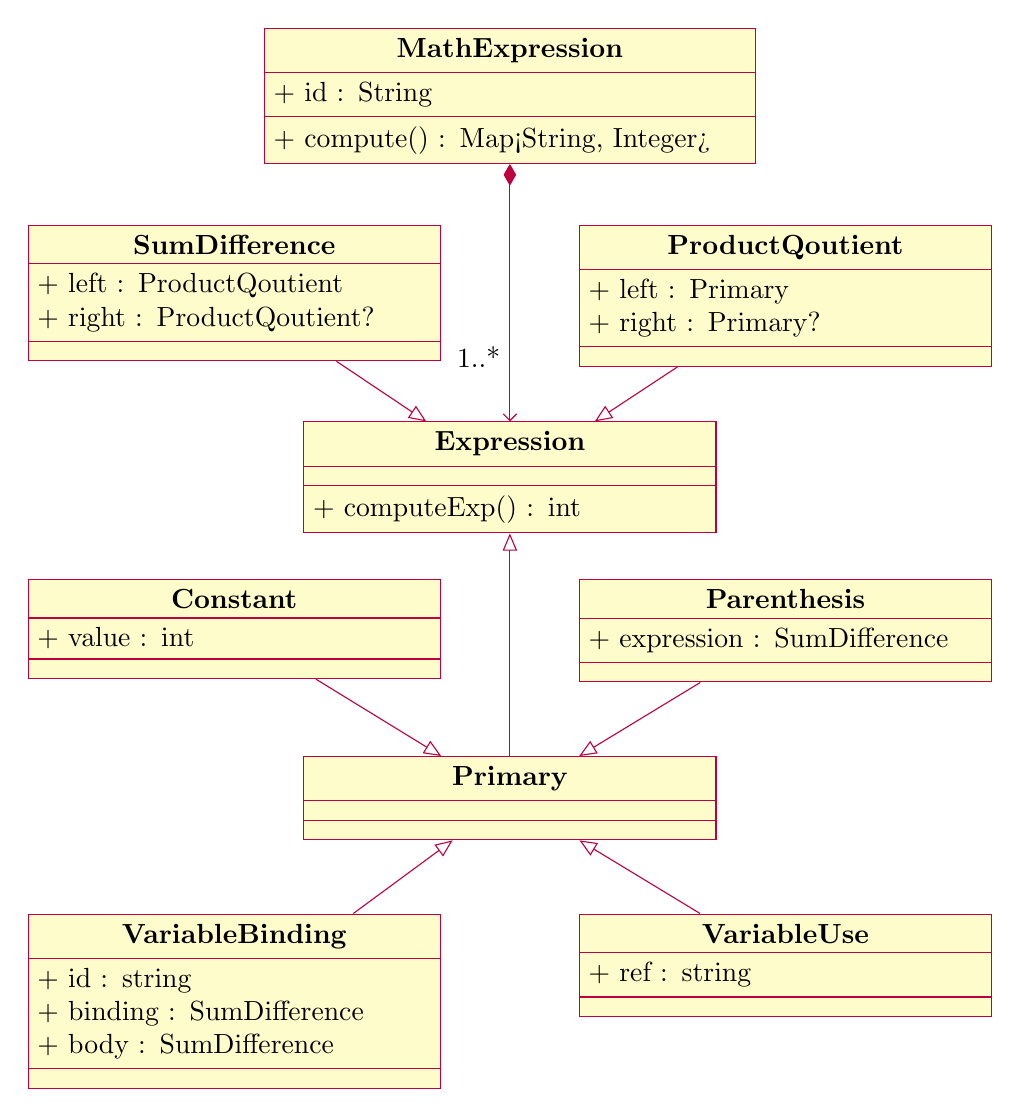
\begin{tikzpicture}
        \begin{class}[text width=6cm]{MathExpression}{0,0}{
            \attribute{+ id : String}
            \operation{+ compute() : Map<String, Integer>}
        }
        \end{class}
        \begin{class}{Expression}{0,-5}{
            \operation{+ computeExp() : int}
        }
        \end{class}
        \begin{class}{SumDifference}{-3.5,-2.5}{
            \attribute{+ left : ProductQoutient}
            \attribute{+ right : ProductQoutient?}
        }
        \inherit{Expression}
        \end{class}
        \begin{class}{ProductQoutient}{3.5,-2.5}{
            \attribute{+ left : Primary}
            \attribute{+ right : Primary?}
        }
        \inherit{Expression}
        \end{class}
        \begin{class}{Primary}{0, -9.25}{
        }
        \inherit{Expression}
        \end{class}
        \begin{class}{Parenthesis}{3.5,-7}{
            \attribute{+ expression : SumDifference}
        }
        \inherit{Primary}
        \end{class}
        \begin{class}{Constant}{-3.5,-7}{
            \attribute{+ value : int}
        }
        \inherit{Primary}
        \end{class}
        \begin{class}{VariableUse}{3.5,-11.25}{
            \attribute{+ ref : string}
        }
        \inherit{Primary}
        \end{class}
        \begin{class}{VariableBinding}{-3.5,-11.25}{
            \attribute{+ id : string}
            \attribute{+ binding : SumDifference}
            \attribute{+ body : SumDifference}
        }
        \inherit{Primary}
        \end{class}
        \composition{MathExpression}{}{1..*}{Expression}
    \end{tikzpicture}
    \caption{Mathematical Expression Metamodel}
    \label{fig:metamoel}
\end{figure}
    

\subsection{Syntax}

The syntax is already given in the different test cases. So, the resulting \textit{XText} grammer has to accommodate syntax as seen in fig.~\ref{lst:syntax}

\begin{center}
    \begin{lstlisting}[language={math}, captionpos={b}, caption={Examples of *.math syntax}, label={lst:syntax}]
        var a = 1
        var b = 1 + 1
        var c = a + b
        var d = let x = 1 + 1 in a end
    \end{lstlisting}
\end{center}

\section{Implmentation}

Repo: \url{https://github.com/Wafl97/MDSD/tree/main/A2/assignment2}

\subsection{XText syntax}
\begin{lstlisting}[caption={XText syntax}, captionpos={b}]
grammar dk.sdu.mmmi.mdsd.Math with org.eclipse.xtext.common.Terminals

generate math "http://www.sdu.dk/mmmi/mdsd/Math"

MathExp:
    exps+=Exp*
;

Exp:
    'var' name=ID '=' exp=SumDiff
;

SumDiff returns Expression:
    ProdQuot (('+'{Add.left=current} | '-'{Sub.left=current}) right=ProdQuot)*
;

ProdQuot returns Expression:
    Primary (('*'{Mul.left=current} | '/'{Div.left=current}) right=Primary)*
;

Primary returns Expression:
    Constant | Parenthesis | VariableUse | VariableBinding
;

Parenthesis returns Expression:
    {Parenthesis} '(' exp=SumDiff ')'
;

Constant returns Expression:
    {Constant} value=INT
;

VariableUse returns Expression:
    {VariableUse} ref=ID
;

VariableBinding returns Expression:
    {VariableBinding} 'let' id=ID '=' binding=SumDiff 'in' body=SumDiff 'end'
;
\end{lstlisting}

\subsection{XTend Generator}
% just the computation code
\begin{lstlisting}[language={xtend}, caption={XTend generator}, captionpos={b}]
override void doGenerate(
    Resource resource, IFileSystemAccess2 fsa, IGeneratorContext context) {
    val variables = resource.allContents.filter(MathExp).next.compute
    
    // You can replace with hovering, see Bettini Chapter 8
    variables.displayPanel
}

def static Map<String, Integer> compute(MathExp math) {
    val variables = new HashMap<String, Integer>()
    
    val tmp = new HashMap<String, Expression>()
    math.exps.forEach[exp | tmp.put(exp.name, exp.exp)]
    
    math.exps.forEach[exp | {
        val res = exp.exp.computeExp(variables, tmp)			
        variables.put(exp.name, res)
    }]
    return variables
}

def static int computeExp(
    Expression exp, Map<String, Integer> vars, Map<String, Expression> tmp) {
    switch exp {
        Add: exp.left.computeExp(vars, tmp)+exp.right.computeExp(vars, tmp)
        Sub: exp.left.computeExp(vars, tmp)-exp.right.computeExp(vars, tmp)
        Mul: exp.left.computeExp(vars, tmp)*exp.right.computeExp(vars, tmp)
        Div: exp.left.computeExp(vars, tmp)/exp.right.computeExp(vars, tmp)
        Constant: exp.value
        Parenthesis: exp.exp.computeExp(vars, tmp)
        VariableUse:
        {
            if (!vars.keySet.contains(exp.ref)) {
                val res = tmp.get(exp.ref).computeExp(vars, tmp)
                vars.put(exp.ref, res)
            }
            vars.get(exp.ref)
        }
        VariableBinding: exp.body.computeExp(
            vars.bind(exp.id, exp.binding.computeExp(vars, tmp)), tmp)
        default: throw new Error("Could not compute expression")
    }
}

def static Map<String, Integer> bind(
    Map<String, Integer> vars, String key, Integer value) {
    val binding = new HashMap<String, Integer>(vars)
    binding.put(key, value)
    binding
}
\end{lstlisting}

\subsection{XTend Validator}

Checking for dublicate var declarations. This is done with a Set, that is cleared when checking the \textbf{MathExp} since it is the first thing that is checked. Hereafter each of the \textbf{Exps} are checked to see if they are in the Set, if yes, then issue a warning and return, if no, add it to the set.

\begin{lstlisting}[language={xtend}, caption={XTend validator}, captionpos={b}]
public static val DUBLICATE_VAR = 'dublicateVar'

val set = new HashSet<String>()

@Check
def clearSet(MathExp m) {
    set.clear
}

@Check
def checkNoDublicateVar(Exp exp) {
    if (set.contains(exp.name)) {
        warning("var " + exp.name + " has already been declared",
            MathPackage.Literals.EXP__NAME,
            DUBLICATE_VAR
        )
        return
    }
    set.add(exp.name)
}
\end{lstlisting}
\section{Test}
% if i can get it to work :)

Current implmentation passes \textbf{MathExampleTest}, \textbf{MathParsingTest}, and \textbf{MathValidatorTest}, but failes \textbf{MathScopeTest}.

\begin{figure}[H]
    \centering
    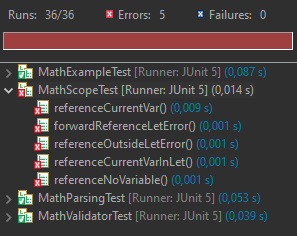
\includegraphics{tests.PNG}
\end{figure}

\section{Conclusion}

The current implementation solves most of the test, however there might be a more elegant solution for solving the \textit{evilExample} test, by using better \textbf{XText} grammer. How it is solved currently feels like a bit of a hack.



\end{document}